\section{Results and Tests}
To test energy consumption during game play, the eAProfiler tool was used.

First, as can be seen in figure \ref{fig:nosleep},
the naive implementation is tested.
This version does not enter sleep mode after rendering a frame,
and contains no framebuffer rendering optimizations.

The high spikes (around $ 35 ma $ ) originate from when the display buffer is
refreshed (\emph{76800} system calls!). This implementation has an average
power consumption of roughly $ 33 ma $. Not very efficient.

\begin{figure}[H]
\centering
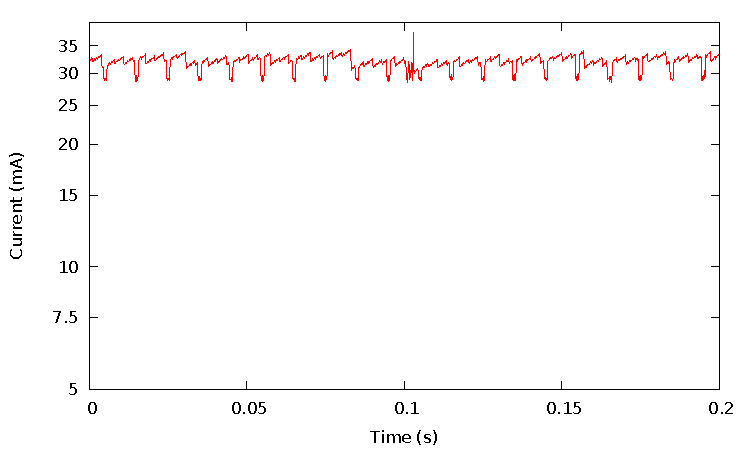
\includegraphics[width=0.7\textwidth]{figures/nosleep.pdf}
\caption{Graph of non sleeping code}
\label{fig:nosleep}
\end{figure}

The interesting thing to see is the comparison to figure
\ref{fig:sleep}, where the device goes to sleep after each
game loop iteration, only waking when it feels the time is
right to draw a new frame.

This version averages $ 29.01 mA $ when awake,
$ 7.59 mA $ when sleeping,
and $ 11.95 mA $ when averaged over 10 seconds.

The fat spikes are from when the framebuffer redraws.
The thin spikes are from kernel ticks.

\begin{figure}[H]
\centering
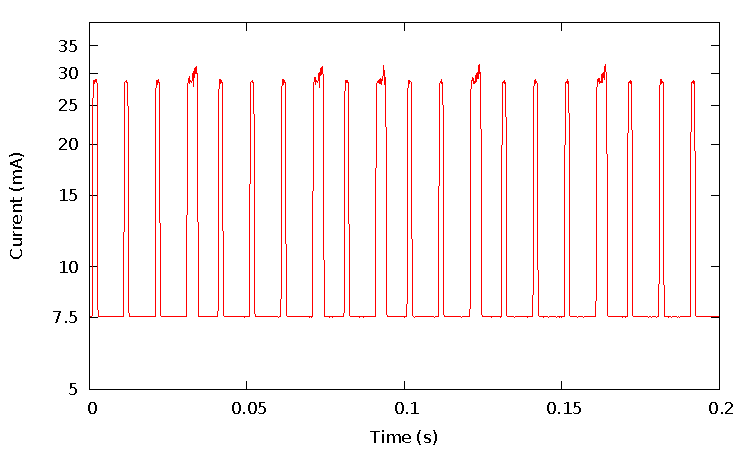
\includegraphics[width=0.7\textwidth]{figures/sleep.pdf}
\caption{Graph of sleeping code}
\label{fig:sleep}
\end{figure}

The power usage of the different implementations are nearly identical at the
peaks, but as shown in figure \ref{fig:sleep}, the energy savings are
considerable.

\subsection{Further improvements}

For increased power savings, kernel ticks can be turned off when the kernel is
idle\footnotemark.

\footnotetext{
  \url{https://www.kernel.org/doc/Documentation/timers/NO_HZ.txt}
}

The Linux kernel offers two modes of tickless running. In the first mode, ticks
are disabled when the CPU. In the second mode, which is available as of kernel
3.10, ticks are also turned off if the CPU is running a single task. While this
newer variant has a more limited suitability, it would be well suited for the
purpose of this project.
